\documentclass[11pt]{article}
\usepackage[margin=1in]{geometry}
\usepackage[T1]{fontenc}
\usepackage{lmodern}
\usepackage{microtype}
\usepackage{amsmath,amssymb}
\usepackage{booktabs,tabularx,array}
\usepackage{enumitem}
\usepackage{xcolor}
\usepackage{listings}
\usepackage{tikz}
\usetikzlibrary{arrows.meta,positioning,calc,fit,shapes.multipart}
\usepackage[obeyspaces,spaces]{url}
\usepackage[hidelinks]{hyperref}

\setlist{itemsep=2pt,topsep=4pt}
\setlength{\parskip}{4pt}
\setlength{\emergencystretch}{3em}
\renewcommand{\arraystretch}{1.2}
\newcolumntype{Y}{>{\raggedright\arraybackslash}X}

\definecolor{codebg}{RGB}{247,247,250}
\definecolor{codeframe}{RGB}{200,200,210}
\definecolor{comment}{RGB}{100,110,120}
\definecolor{keyword}{RGB}{30,60,140}
\definecolor{string}{RGB}{150,60,20}
\definecolor{notebg}{RGB}{238,244,252}
\definecolor{warnbg}{RGB}{253,240,232}
\definecolor{lapi}{RGB}{225,238,252}
\definecolor{leng}{RGB}{230,245,232}
\definecolor{lms4}{RGB}{252,243,224}
\definecolor{lcore}{RGB}{238,238,238}

\lstdefinestyle{java}{language=Java, basicstyle=\ttfamily\small, columns=fullflexible, keepspaces=true,
  keywordstyle=\color{keyword}\bfseries, commentstyle=\color{comment}\itshape, stringstyle=\color{string},
  backgroundcolor=\color{codebg}, frame=single, rulecolor=\color{codeframe}, breaklines=true,
  showstringspaces=false, xleftmargin=4pt, xrightmargin=4pt, aboveskip=6pt, belowskip=6pt}
\lstset{style=java}

\newcommand{\code}[1]{\texttt{#1}}
\newcommand{\note}[1]{\par\noindent\colorbox{notebg}{\parbox{\dimexpr\linewidth-2\fboxsep}{\small\textbf{Note.} #1}}\par}
\newcommand{\warn}[1]{\par\noindent\colorbox{warnbg}{\parbox{\dimexpr\linewidth-2\fboxsep}{\small\textbf{Caution.} #1}}\par}

\tikzset{box/.style={draw,rounded corners=2pt,align=center,inner sep=4pt,font=\small},
  flow/.style={-{Latex[length=2mm]},thick}, dflow/.style={-{Latex[length=2mm]},thick,dashed},
  lbl/.style={font=\footnotesize,fill=white,inner sep=1.5pt}}

\title{\textbf{ParaDEVS Library}\\[4pt]\large Architecture and Interpretation Guide (library v0)}
\author{ParaDEVS Library workspace, Binghamton}
\date{October 9, 2026}

\newcommand{\docsdir}{../}
\def\thisdoc{architecture}
% Shared cross-document links for the ParaDEVS documents. Each document defines \docsdir (path from its folder to
% docs/) and \thisdoc (its key below), then \input's this file.
%
% \doclink{path relative to docs/}{text}: a link to another PDF. Links are plain URI actions (file:///...), because
% Edge, Chrome and VS Code's PDF viewers ignore hyperref's usual "open another PDF" (GoToR) links. The absolute
% address comes from docroot.tex, which scripts/build_docs.sh regenerates; rerun it if the folder moves.
%
% \relateddocs: the "ParaDEVS documents" box listing every document, with the current one marked.
\InputIfFileExists{\docsdir docroot.tex}{}{\gdef\docroot{.}}
\providecommand{\thisdoc}{}
\definecolor{pdlink}{RGB}{20,80,170}
\definecolor{pdrelbg}{RGB}{243,246,252}
\definecolor{pdrelframe}{RGB}{190,200,220}
\makeatletter
\newcommand{\doclink}[2]{\hyper@linkurl{\textcolor{pdlink}{\textbf{#2}}}{\docroot/#1}}
\newcommand{\pd@item}[4]{% key, path, title, description
  \def\pd@key{#1}%
  \item \ifx\pd@key\thisdoc\textbf{#3} (this document)\else\doclink{#2}{#3}\fi: #4}
\newcommand{\relateddocs}{\par\medskip\noindent
  \fcolorbox{pdrelframe}{pdrelbg}{\parbox{\dimexpr\linewidth-2\fboxsep-2\fboxrule}{\small
  \textbf{ParaDEVS documents.} The entry point is \doclink{ParaDEVS_Start_Here.pdf}{Start Here}, a reading guide
  that links every document.
  \begin{itemize}[leftmargin=1.4em,itemsep=0pt,topsep=2pt]
  \pd@item{report}{report/ParaDEVS_Build_Report.pdf}{Build Report}{what has been built, how it was verified, what is next}
  \pd@item{howto}{howto/ParaDEVS_HowTo.pdf}{How-To Guide}{setup, tutorials, API reference, troubleshooting}
  \pd@item{architecture}{architecture/ParaDEVS_Architecture.pdf}{Architecture Guide}{how the library works and how to read results}
  \pd@item{rl}{rl/ParaDEVS_RL_Plan.pdf}{RL Plan}{reinforcement-learning plan, analysis and results}
  \pd@item{control}{rl/ParaDEVS_Control_Spec.pdf}{Control Spec}{action selection: Para.decide, graph-mode planning, value and policy iteration}
  \pd@item{hybrid}{rl/ParaDEVS_Hybrid_Study.pdf}{Hybrid Study}{which draws to enumerate or sample, and how cost grows with lookahead}
  \pd@item{fastcopy}{engine/ParaDEVS_FastCopy_Proposal.pdf}{Fast-Copy Proposal}{why the engine replays steps, where time goes, how to speed it up}
  \end{itemize}}}\par\medskip}
\makeatother


\begin{document}
\maketitle

\begin{abstract}
\noindent This document explains how the ParaDEVS library is built and how its results should be read. It is a
companion to the \doclink{howto/ParaDEVS_HowTo.pdf}{How-To Guide}, which covers \emph{how to use} the library. Here we describe
the layers and their contracts, how the engine drives MS4 models, the life of a branch from one event to the next,
what each number in a result means under each selection rule, which guarantees from the theory hold and under which
conditions, and where the design is meant to be extended. The theory referred to throughout is
\path{main_paratemporal.tex} and \path{Paratemporal_Adaptation.tex} in \path{Do s/documents/paratemporal}.
\end{abstract}

\relateddocs

\tableofcontents
\newpage

%=====================================================================
\section{Purpose and design principles}

The library turns an ordinary stochastic MS4 DEVS model into a \emph{paratemporal} computation: whenever the model
makes a random choice, the engine follows the possible outcomes and weights them, and it returns the resulting
distribution over what the experiment observes. The design follows five principles.

\begin{enumerate}[label=\textbf{P\arabic*.}]
\item \textbf{One model-side call.} A model's only obligation is to obtain random values through
  \code{Para.choose(label, law)}. Otherwise it is an ordinary MS4 model, and it still runs under MS4's own simulator.
\item \textbf{The engine owns randomness.} Models never decide how a choice is explored. The engine decides,
  through a \emph{selection rule}: all outcomes, a sample, or a pruned subset. This is the paper's split between model
  and engine: ``the model identifies the missing value and its conditional law, and the engine selects its possible
  values and assigns their weights.''
\item \textbf{Branch at the draw.} The engine branches each time the model calls \code{Para.choose}: one random value
  inside a DEVS transition. It does not branch on a whole ``step'', nor on a whole transition. The old tree engines
  treated a step, a draw, a batch of DEVS events and a tree level as the same thing. The library keeps them separate
  (Section~\ref{sec:stepdraw}).
\item \textbf{One clock.} All branches advance on one simulated clock. Branching takes no simulated time
  (Adaptation, decision D1).
\item \textbf{Never trade correctness for size silently.} Merging is \emph{safe} (complete-state keys only),
  pruning is accounted for in an explicit residual, and combinations that defeat an estimator are refused.
\end{enumerate}

\subsection{Step versus draw (principle P3 in detail)}
\label{sec:stepdraw}

\paragraph{What the old engines did.} In FinanceDEVS and BaseballDEVS, the unit of work was a \emph{step}: one level
of the tree. For each leaf and each outcome in a hard-coded list (\code{Buy/Sell/Holding}, \code{YrOut}\dots\code{Walk}),
the engine rebuilt the coupled model, injected the outcome and the saved state by reflection, ran the simulation for
several DEVS events (\code{Activate} $\to$ \code{GenerateCall} $\to$ the portfolio's external transition), and read the
probability back out of a message. Four different things were bundled into that one unit:

\begin{center}
\small
\begin{tabularx}{\linewidth}{@{}>{\raggedright\arraybackslash}p{5.2cm} >{\raggedright\arraybackslash}p{3.2cm} Y@{}}
\toprule
\textbf{Bundled into one old ``step''} & \textbf{What it really is} & \textbf{In the library}\\
\midrule
one tree level (\code{GeneralTree.depth}) & exploration structure & No depth. A run ends by the stop rules: horizon, acceptor, or passive.\\
one random outcome, chosen \emph{outside} the model from a fixed list & a draw & A call to \code{Para.choose} \emph{inside} the model, wherever the randomness actually is.\\
one simulation run to a maximum time & several DEVS events & Time advances event by event on one clock. Many events can pass with no branching.\\
one save/restore of state (\code{GeneralNode} $\leftrightarrow$ \code{setValue}) & a branch copy & An internal mechanism with no modelling meaning.\\
\bottomrule
\end{tabularx}
\end{center}
They could be treated as one because every old step contained exactly one random choice. As soon as a model has an event
with no randomness, or an event with two random values, they come apart.

\paragraph{Draws are finer than transitions.} One DEVS transition can contain several draws, and a later draw's law can
depend on an earlier value. In the timed reward model a single external transition does
\begin{lstlisting}
int qn = Para.choose("phase",  nextPhase(qPrev));       // P(q' | q)
int r  = Para.choose("reward", rewardLaw(qPrev, qn));   // P(r | q, q'): uses qn
\end{lstlisting}
\begin{itemize}
\item \textbf{Branching on the whole transition} (as in the V12 formalization) treats it as one random event with a
  joint law over next states, $P(s' \mid s, e, x)$. Here the model would have to supply the 4-outcome table
  $P(q', r \mid q)$, computed in advance.
\item \textbf{Branching on each draw} (the current theory; Adaptation, conflict C1) splits at the first draw. Each child
  resumes the \emph{same} transition with $q'$ fixed and splits again at the second draw. The engine produces the same
  4 children with weights $P(q'\mid q)\,P(r \mid q, q')$, and the model never states the joint law.
\end{itemize}
The same holds in coupled models: if two components are imminent at the same instant and each draws, that is one
transition of the coupled model with two draws in two components. Draw-level branching handles it with no extra work.

\paragraph{When they coincide.} If an event makes exactly one draw, branching on the draw and branching on the
transition are the same. That is the case in the finance and baseball ports, so there P3 changes no numbers. It
matters for dependent draws within one event, for simultaneous draws in coupled models, for draws in
\code{initialize()}, and for events with no draw at all.

\paragraph{Why the theory insists on draws.} A suspended branch only ever needs the conditional law of the
\emph{next} missing value, whose inputs are already known. That is what makes ``copy the realized past, supply the
next value, resume'' correct (Adaptation, Proposition ``Restart sufficiency''), and it is exactly what the library's
replay does (Section~\ref{sec:replay}).

%=====================================================================
\section{Layered structure}

\begin{figure}[h]
\centering
\begin{tikzpicture}[node distance=3mm]
\node[box,fill=lapi,minimum width=13.6cm,text width=13.2cm] (user) {\textbf{User code}\\
  MS4 models (atomic \code{AtomicModelImpl} / coupled \code{CoupledModelImpl}) that call \code{Para.choose};
  experiment drivers that build a \code{ParaSpec} and read a \code{ParaResult}};
\node[box,fill=lapi,minimum width=5.6cm,text width=5.3cm,minimum height=1.9cm,below=7mm of user.south west,anchor=north west] (api)
  {\textbf{Model API}\\\code{paradevs}\\\code{Para}, \code{Law},\\\code{Para.DrawContext}, \code{Para.Suspension}};
\node[box,fill=leng,minimum width=5.6cm,text width=5.3cm,minimum height=1.9cm,below=7mm of user.south east,anchor=north east] (eng)
  {\textbf{Engine}\\\code{paradevs.engine}\\\code{ParaEngine}, \code{ParaSpec}, \code{ParaResult},\\
  \code{SelectionRule}, \code{Transducer}, \code{InputTrace}};
\node[box,fill=lms4,minimum width=13.6cm,text width=13.2cm,anchor=north] (ms4) at ($(user.south)+(0,-4.1)$)
  {\textbf{MS4 adapter} \quad \code{paradevs.ms4}\\\code{ModelNode} (atomic driver + ordered coupled coordinator),
  \code{Snapshots} (copy/restore), \code{StateKeys} (complete-state merge keys)};
\node[box,fill=lcore,minimum width=13.6cm,text width=13.2cm,below=7mm of ms4] (core)
  {\textbf{MS4 DEVS core} \quad \code{com.ms4systems.devs.core} (from \path{lib/ms4-core.jar} or the MS4 Me jars)\\
  \code{AtomicModelImpl}, \code{SimulatorImpl}, \code{CoupledModelImpl}, \code{Coupling}, \code{Port}, \code{MessageBag}};
\draw[flow] (user.south -| api.north) -- (api.north);
\draw[flow] (user.south -| eng.north) -- (eng.north);
\draw[flow] (eng.south) -- (eng.south |- ms4.north);
\draw[dflow] (eng.west) -- (api.east);
\draw[flow] (ms4.south) -- (core.north);
\end{tikzpicture}
\caption{Layers and allowed dependencies (arrows point to what a layer uses). Models depend only on the Model API
and on the MS4 core directly. The Model API knows nothing about the engine: the engine reaches it only by installing a
thread-local draw context (dashed). The MS4 adapter is the only engine-side code that touches MS4 internals.}
\label{fig:layers}
\end{figure}

\begin{center}
\small
\begin{tabularx}{\linewidth}{@{}>{\bfseries}p{2.3cm} p{3.6cm} Y@{}}
\toprule
Layer & Classes (lines) & Responsibility and contract\\
\midrule
Model API & \code{Law} (118), \code{Para} (101) &
  \code{Law}: a finite, ordered, validated discrete law (mass 1 within $10^{-6}$, zero atoms dropped).
  \code{Para.choose}: samples when no engine is active; under the engine, returns the next supplied value or
  suspends the running transition. No dependency on the engine.\\
Engine & \code{ParaEngine} (285), \code{ParaSpec} (58), \code{ParaResult} (72), \code{SelectionRule} (70),
  \code{Transducer} (60), \code{InputTrace} (55), \code{OutputEvent}, \code{StopStatus} &
  The paper's algorithm: roots, $\Gamma_{\mathrm{PT}}$, \textsc{Advance}, \textsc{doExpansion}, \textsc{RunLocal},
  \textsc{StopStatus}, merge, collector. Domain-free: knows nothing about finance or baseball.\\
MS4 adapter & \code{ModelNode} (156), \code{Snapshots} (47), \code{StateKeys} (111) &
  Runs one Parallel DEVS event on an MS4 model; copies and restores the complete model graph; computes the canonical
  complete state for merging.\\
MS4 core & external &
  Unchanged. Atomic models are driven through their own \code{SimulatorImpl}.\\
\bottomrule
\end{tabularx}
\end{center}

\paragraph{Why this split.} The model API must be importable by any MS4 model, including DNL-generated code, without
pulling in the engine, so that the same model runs under MS4 Me unchanged (P1). All MS4-specific behaviour (event
times, couplings, serialization quirks) is isolated in the adapter, so the engine reads like the paper's pseudocode and
could be pointed at another DEVS kernel by replacing one package.

%=====================================================================
\section{Integration with MS4}

\subsection{Driving an atomic model}
\code{ModelNode.Atomic} wraps a model and its own MS4 \code{SimulatorImpl} (every \code{AtomicModelImpl} creates one).
One event is run with MS4's own methods, so model code that calls \code{getSimulator()} (for the current time,
\code{holdIn} messages) behaves exactly as under MS4:
\begin{center}
\small
\begin{tabularx}{\linewidth}{@{}p{2.7cm} Y@{}}
\toprule
\textbf{Event} & \textbf{MS4 calls made}\\
\midrule
initial & \code{sim.initialize(0)}: calls the model's \code{initialize()} (MS4 does this only at time 0), sets $t_L$, $t_N$\\
internal at $t$ & \code{sim.computeOutput()} $\to$ outputs; \code{sim.executeNextEvent(t)}\\
external at $t$ & \code{sim.processInput(t, bag)}: MS4 calls \code{externalTransition(e, bag)} with $e = t - t_L$\\
confluent at $t$ & \code{sim.computeOutput()} $\to$ outputs; \code{sim.processInput(t, bag)}: MS4 calls \code{confluentTransition}\\
\bottomrule
\end{tabularx}
\end{center}

\subsection{Driving a coupled model: the ordered coordinator}
MS4's \code{CoordinatorImpl} routes messages through \code{HashMap}s keyed by simulator objects with identity hash
codes. The order in which it processes simultaneous children can therefore differ between two copies of the same
model. The engine replays transitions (Section~\ref{sec:replay}), and a replay must request the same draws in the same
order, so the library does not use MS4's coordinator. \code{ModelNode.Coupled} is a small Parallel DEVS coordinator
with a fixed order:

\begin{figure}[h]
\centering
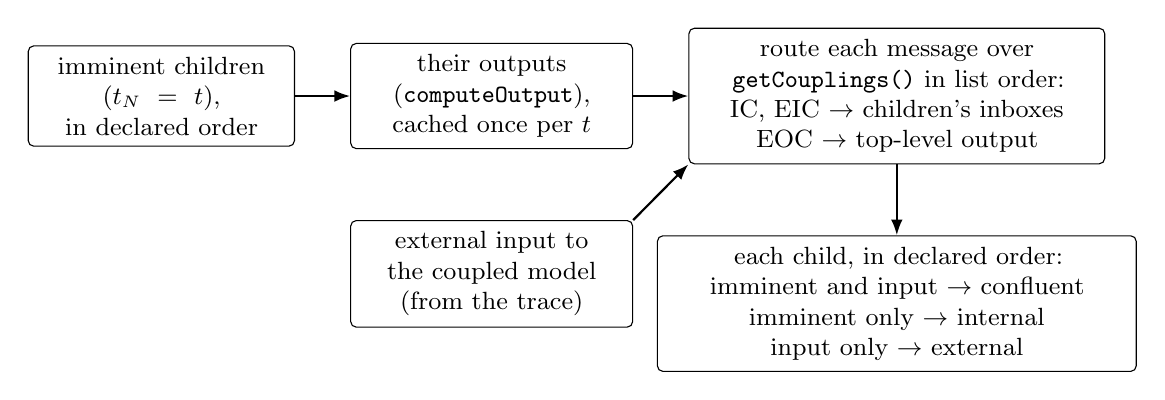
\begin{tikzpicture}[node distance=6mm and 7mm]
\node[box,text width=3.1cm] (imm) {imminent children\\($t_N = t$),\\in declared order};
\node[box,text width=3.3cm,right=of imm] (out) {their outputs\\(\code{computeOutput}),\\cached once per $t$};
\node[box,text width=5.0cm,right=of out] (route) {route each message over\\\code{getCouplings()} in list order:\\IC, EIC $\to$ children's inboxes\\EOC $\to$ top-level output};
\node[box,text width=5.8cm,below=9mm of route] (tr) {each child, in declared order:\\imminent and input $\to$ confluent\\imminent only $\to$ internal\\input only $\to$ external};
\node[box,text width=3.3cm,below=9mm of out] (ext) {external input to\\the coupled model\\(from the trace)};
\draw[flow] (imm) -- (out); \draw[flow] (out) -- (route); \draw[flow] (route) -- (tr);
\draw[flow] (ext.north east) -- (route.south west);
\end{tikzpicture}
\caption{One event of a coupled model. Children and couplings are visited in their declared list order, which is the
order of \code{addChildModel} and \code{addCoupling} calls (or the SES/PES-generated \code{make()}).}
\label{fig:coord}
\end{figure}

Nested coupled models are handled recursively. Atomic children are still driven by their own MS4 \code{SimulatorImpl}.
Only the top model's outputs, reached through external output couplings, are observed by the experiment.

\subsection{Copying and restoring branches}
A branch's model state is stored as the Java-serialized bytes of the \emph{whole} model graph, including ports, MS4
simulators with their event times $t_L, t_N$, children and couplings (\code{Snapshots.save}). Copying a branch shares
the bytes; running it restores an independent graph (\code{Snapshots.restore}). This is generic: any MS4 model whose
fields are \code{Serializable} works, and nothing is read through model-specific accessors. It realizes the paper's
restart requirement (Adaptation, Proposition ``Restart sufficiency''): at a persistent boundary, the retained state and
the event times are enough to continue with the correct law.

\subsection{Complete-state keys for merging}
\code{StateKeys.of(model)} builds a canonical value for the state. For each atomic model, in declared order, it
records the class, name, MS4 $t_L$ and $t_N$, and \emph{every} instance field declared by the model's own classes,
including bookkeeping such as \code{phase}, \code{sigma}, \code{currentTime}, \code{previousPhase}. Excluded are only
structural references that are identical in every copy: ports, simulators, parent/child models,
\code{PropertyChangeSupport}, MS4 helper options. Values are compared by \code{equals} when the class overrides it,
otherwise by serialized bytes, otherwise by identity. Every fallback can only \emph{prevent} a merge, never cause a wrong
one. A model may supply its own key (\code{StateKeys.ParaStateKey}), and is then responsible for its completeness.

%=====================================================================
\section{Execution model}

\subsection{The records}
\begin{center}
\small
\begin{tabularx}{\linewidth}{@{}>{\ttfamily}p{2.8cm} p{4.4cm} Y@{}}
\toprule
\normalfont\textbf{Record} & \textbf{Fields} & \textbf{Role (paper name)}\\
\midrule
Branch & state bytes, key, $\theta$, $t_N$, $j$, $n$, $\xi$, $w$ &
  A live persistent branch $k=(\eta,t,\theta,j,n,\xi,w)$. $\theta$: time of its last persistent entry; $t_N$: model's
  next internal event; $j$: input-trace cursor; $n$: entry count; $\xi$: observation; $w$: weight.\\
Continuation & parent Branch, event kind and time, supplied values, pending draw, $w$ &
  A departure suspended at a choice point: the payload $\rho$ of a choice request.\\
Request & branch name; stop status \emph{or} continuation & What one simulator step asks of $\Gamma_{\mathrm{PT}}$.\\
ParaResult & collector, residual, stats & The collector $\widehat\mu=\sum_k w_k\delta_{(\xi_k,h_k)}$ and the omitted mass $r$.\\
\bottomrule
\end{tabularx}
\end{center}
Live branches are kept in a \code{TreeMap} by name. Requests are resolved in name order and new branches get fresh,
increasing names, so a run is fully deterministic for a given seed.

\subsection{The main loop}
\begin{enumerate}
\item \textbf{Roots.} Serialize a fresh (uninitialized) model from the factory. Run its \code{initialize()} as the first
  departure under the selection rule, $N$ times with weight $1/N$ each (Monte Carlo) or once with weight 1. Draws in
  \code{initialize()} branch like any other draw. Apply \textsc{StopStatus}, merge, install.
\item \textbf{Repeat while live branches remain:}
  \begin{enumerate}
  \item $\Gamma_{\mathrm{PT}}$: resolve the requests from the previous step (stops are collected, choices expanded),
    remove their parents, merge the new children, install them.
  \item Choose $t=\min_k \mathrm{NextTime}(k)$, where $\mathrm{NextTime}(k)=\min(t_N, \text{time of trace entry } j)$.
  \item \textsc{Advance} every branch with $\mathrm{NextTime}=t$, in name order. A branch that completes its event without
    a non-degenerate draw is updated in place; one that hits a draw or a stop condition files a request.
  \end{enumerate}
\end{enumerate}
The event type is decided per branch: external if the next input comes first, internal if $t_N$ comes first,
confluent if they coincide.

\subsection{Life of a branch}
\begin{figure}[h]
\centering
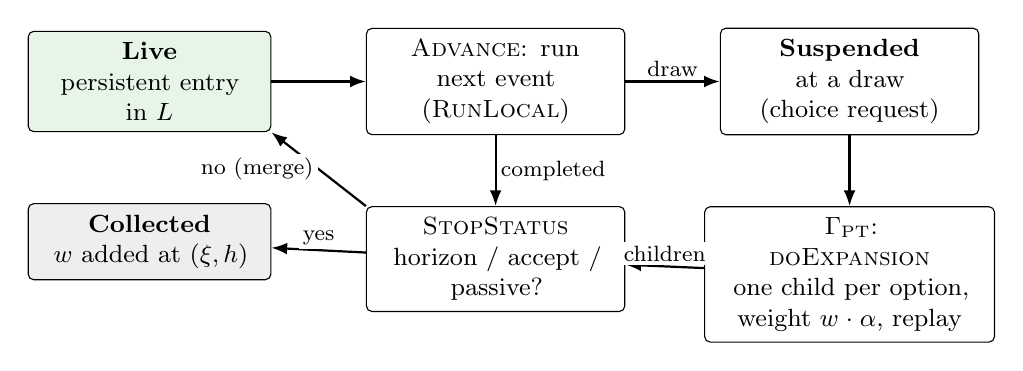
\begin{tikzpicture}[node distance=9mm and 12mm]
\node[box,fill=leng,text width=2.8cm] (live) {\textbf{Live}\\persistent entry\\in $L$};
\node[box,text width=3.0cm,right=of live] (run) {\textsc{Advance}: run\\next event\\(\textsc{RunLocal})};
\node[box,text width=3.0cm,right=of run] (susp) {\textbf{Suspended}\\at a draw\\(choice request)};
\node[box,text width=3.4cm,below=of susp] (exp) {$\Gamma_{\mathrm{PT}}$:\\\textsc{doExpansion}\\one child per option,\\weight $w\cdot\alpha$, replay};
\node[box,text width=3.0cm,below=of run] (stop) {\textsc{StopStatus}\\horizon / accept /\\passive?};
\node[box,fill=lcore,text width=2.8cm,below=of live] (done) {\textbf{Collected}\\$w$ added at $(\xi,h)$};
\draw[flow] (live) -- (run);
\draw[flow] (run) -- node[lbl,above]{draw} (susp);
\draw[flow] (susp) -- (exp);
\draw[flow] (exp) -- node[lbl,above]{children} (stop);
\draw[flow] (run) -- node[lbl,right]{completed} (stop);
\draw[flow] (stop) -- node[lbl,above]{yes} (done);
\draw[flow] (stop.north west) -- node[lbl,left]{no (merge)} (live.south east);
\end{tikzpicture}
\caption{States of a branch. A suspended parent stays in $L$ until $\Gamma_{\mathrm{PT}}$ replaces it, so its weight is
always accounted for exactly once.}
\label{fig:life}
\end{figure}

\subsection{Suspension and replay}
\label{sec:replay}
Java cannot pause a method in the middle and resume it later, so the library uses the paper's \emph{derandomized
departure} (Adaptation, Definition 5.1): an event is a deterministic function of the persistent state, the event
arguments, and the drawn values $v_1,\dots,v_N$.

\begin{figure}[h]
\centering
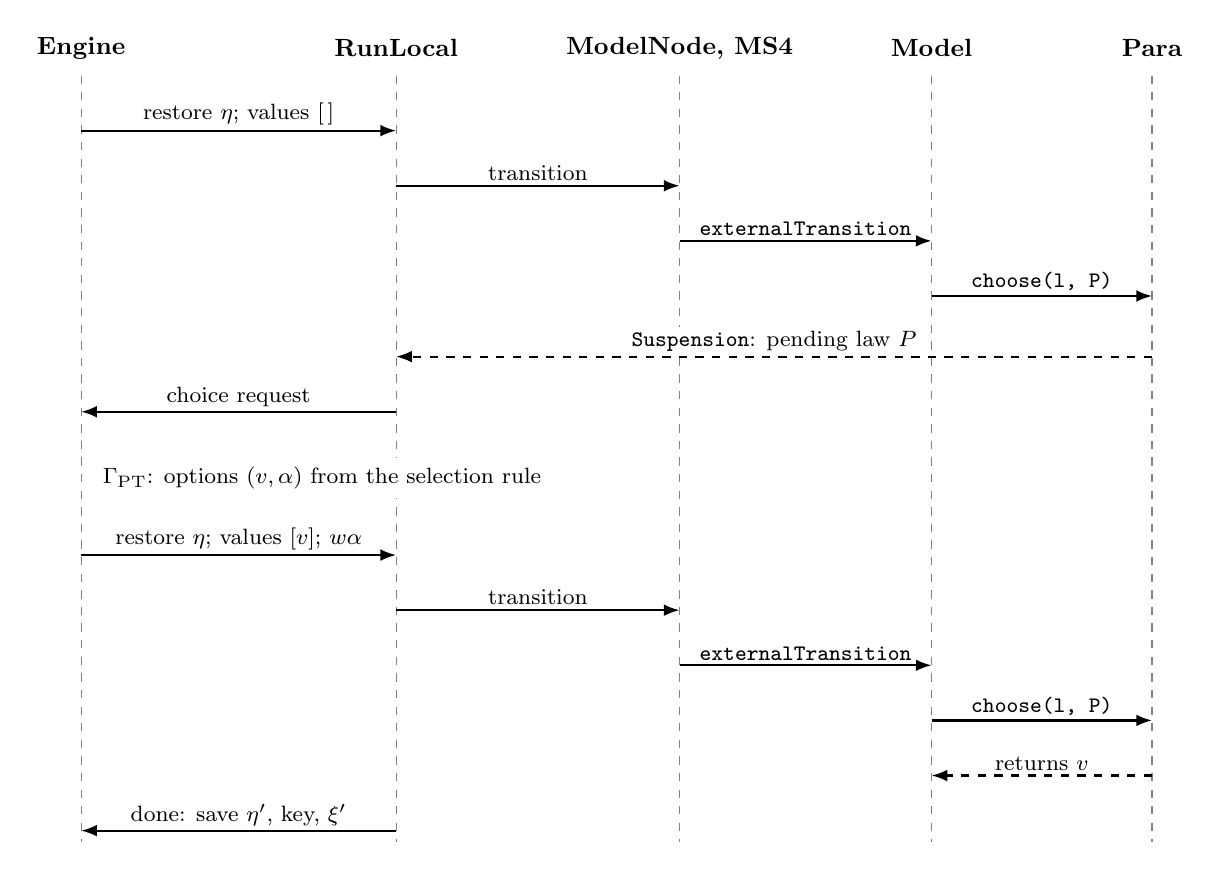
\begin{tikzpicture}[x=1cm,y=-0.7cm,font=\small]
\foreach \x/\name in {0/Engine,4.0/RunLocal,7.6/{ModelNode, MS4},10.8/Model,13.6/Para}
  { \node[font=\small\bfseries] at (\x,0) {\name}; \draw[gray,dashed] (\x,0.5) -- (\x,14.4); }
\draw[flow] (0,1.5) -- node[lbl,above]{restore $\eta$; values $[\,]$} (4.0,1.5);
\draw[flow] (4.0,2.5) -- node[lbl,above]{transition} (7.6,2.5);
\draw[flow] (7.6,3.5) -- node[lbl,above]{\code{externalTransition}} (10.8,3.5);
\draw[flow] (10.8,4.5) -- node[lbl,above]{\code{choose(l, P)}} (13.6,4.5);
\draw[dflow] (13.6,5.6) -- node[lbl,above]{\code{Suspension}: pending law $P$} (4.0,5.6);
\draw[flow] (4.0,6.6) -- node[lbl,above]{choice request} (0,6.6);
\node[align=left,anchor=west,font=\footnotesize,fill=white] at (0.15,7.8) {$\Gamma_{\mathrm{PT}}$: options $(v,\alpha)$ from the selection rule};
\draw[flow] (0,9.2) -- node[lbl,above]{restore $\eta$; values $[v]$; $w\alpha$} (4.0,9.2);
\draw[flow] (4.0,10.2) -- node[lbl,above]{transition} (7.6,10.2);
\draw[flow] (7.6,11.2) -- node[lbl,above]{\code{externalTransition}} (10.8,11.2);
\draw[flow] (10.8,12.2) -- node[lbl,above]{\code{choose(l, P)}} (13.6,12.2);
\draw[dflow] (13.6,13.2) -- node[lbl,above]{returns $v$} (10.8,13.2);
\draw[flow] (4.0,14.2) -- node[lbl,above]{done: save $\eta'$, key, $\xi'$} (0,14.2);
\end{tikzpicture}
\caption{One draw, end to end. The first run discovers the pending law; each child re-runs the event from the same
saved state with one more supplied value. A second draw in the same event repeats the pattern with two supplied values.}
\label{fig:seq}
\end{figure}

Consequences:
\begin{itemize}
\item \textbf{Each requested value is written once and realized values are reused}, as \textsc{RunLocal} requires:
  earlier draws in the same event are replayed from the supplied list, never redrawn.
\item \textbf{Determinism is checked}: a replayed draw whose supplied value is not in the law it now sees, or a
  replay that uses fewer values than supplied, raises an error naming the draw.
\item \textbf{Laws with a single outcome never suspend} (\textsc{RunLocal} passes through degenerate draws).
\item \textbf{Cost}: an event with $D$ draws and $b$ options each is run $1 + b + b^2 + \dots + b^D$ times. The statistic
  \code{departures} counts all runs, including replays.
\end{itemize}

\subsection{What \textsc{RunLocal} does after an event completes}
In this order: advance the trace cursor if an input was consumed; fold the event's outputs into $\xi$ with the
transducer (called for every completed event, with an empty list when there was no output); compute the state key (only
when merging); serialize the model; record $\theta=t$, the new $t_N$, and $n+1$.

\subsection{Stopping}
\textsc{StopStatus} is applied to roots and to every completed entry, in the paper's order:
\begin{enumerate}
\item \code{HORIZON} if $n \ge m$ (the initial state is entry 1);
\item \code{ACCEPT} if the acceptor returns true for $(\xi, \theta, n)$;
\item \code{PASSIVE} if $t_N=\infty$ and the trace is exhausted;
\item otherwise \code{LIVE}. An infinite time advance alone is not terminal while inputs remain.
\end{enumerate}

\subsection{Merging}
Under \code{Merge.SAFE}, the children produced by one $\Gamma_{\mathrm{PT}}$ update (and the roots) are grouped by the key
$(\text{state key}, \theta, j, n, \xi)$. Each group is replaced by its first member carrying the summed weight. This is the
complete continuation key of the paper's Proposition ``Safe merging'', and merging stays local to the update, as the
paper prescribes.

\paragraph{Expectation-only merging (opt-in).} \code{Merge.EXPECTATION} is off by default and needs a transducer that
implements \code{Transducer.Additive}, which splits $\xi=(G,\text{rest})$ into an additive accumulated reward
$G=\code{reward}(\xi)$ and the rest, with \code{withReward}$(\xi,r)$ replacing $G$. The key is
$(\text{state key}, \theta, j, n, \text{rest})$, with the reward zeroed. A group of weights $w_i$ and rewards $G_i$ becomes one
record of weight $W=\sum_i w_i$ and reward $A/W$, $A=\sum_i w_i G_i$. The members share their future, so by linearity
$E[G]=\sum_s A_s+\sum_s W_s\,E[G_{\text{future}}\mid s]$ is unchanged, and so is $E[a(\text{rest})\,G+b(\text{rest})]$ for
any functions $a$, $b$. The law of $G$ is lost. The result therefore refuses \code{distribution()}, \code{marginal(g)} and
the general \code{expectation(f)} with an \code{IllegalStateException}, and answers \code{expectation(slope, offset)}, which
evaluates $\sum w\,(\text{slope}(\text{rest})\,G+\text{offset}(\text{rest}))$, and \code{expectedReward()}. Both functions
receive only the rest, so the rule holds by construction. The transducer's contract: the increment that \code{record} adds
to $G$, and the new rest, do not depend on $G$, and the acceptor ignores $G$. The mode is valid only for linear objectives
with additive rewards; it is refused without \code{Additive} and with $N>1$ roots.

%=====================================================================
\section{Interpreting results}

\subsection{What the result is a distribution of}
A \code{ParaResult} is a measure over pairs $(\xi, h)$: the \emph{observation} the transducer built from the top
model's outputs, and the \emph{stop status}. Three things follow.
\begin{itemize}
\item It is a distribution of what you chose to observe, at the moment each branch stopped. Internal state that never
  leaves the model through a port is invisible. Couple it out if you need it.
\item Branches may stop for different reasons. Read the status: mixing \code{HORIZON} leaves (stopped mid-run) with
  \code{PASSIVE} leaves (finished) is legitimate but answers a mixed question. Filter by status, or design the
  experiment so that all branches stop for the same reason.
\item Weights are exact path probabilities (exhaustive) or estimator weights (sampling). They are \emph{not}
  frequencies of a single simulation.
\end{itemize}

\subsection{By selection rule}
\begin{center}
\small
\begin{tabularx}{\linewidth}{@{}>{\bfseries}p{2.4cm} Y Y@{}}
\toprule
Rule & What \code{distribution()} and \code{expectation(f)} are & Checks and uncertainty\\
\midrule
Exhaustive & The exact terminal law and exact expectations (up to floating point, about $10^{-12}$ relative in the tests). &
  \code{totalMass()} $=1$. A different value means a law in the model (or its data) is not proper; see below.\\
Partial ($p_{\min}$) & A lower bound: each event probability $P(E)$ satisfies
  $\widehat\mu(E)\le P(E)\le\widehat\mu(E)+r$ with $r=$ \code{residual()}. &
  \code{totalMass()} $+$ \code{residual()} $=1$. Expectations of bounded $f$ are bracketed in the same way
  by $\pm r\cdot\sup|f|$.\\
Monte Carlo ($N$ roots) & An unbiased estimate; each root contributes weight $1/N$ to one sampled outcome. &
  \code{totalMass()} $=1$ exactly. Standard error of an event probability is $\sqrt{p(1-p)/N}$.
  Repeat with other seeds to see the spread.\\
Hybrid & Exact over the exhaustively treated draws, unbiased over the sampled ones. & As for Monte Carlo, on the sampled part.\\
\bottomrule
\end{tabularx}
\end{center}

\subsection{Total mass different from 1}
With proper laws and exhaustive selection the mass is 1. It differs only when a law was built with
\code{Law.asGiven(\dots, tol)} from data whose rows do not sum to 1. Example: baseball's mass is $1.000131$ because one
source row sums to $1.0004$. The result is then exactly what the data implies, which is what reproducing an old engine
requires. For a probability statement about the data-generating process, either fix the data or divide by the mass.
Both change the question slightly; record which one you used.

\subsection{Stats: reading cost, not results}
\begin{center}
\small
\begin{tabularx}{\linewidth}{@{}>{\ttfamily}p{2.6cm} Y@{}}
\toprule
\normalfont\textbf{Stat} & \textbf{Meaning}\\
\midrule
leaves & Terminal branches collected (before equal outcomes are summed). \code{distribution().size()} is the number of distinct outcomes.\\
choiceNodes & Non-degenerate draws expanded (the paper's ``random choice nodes'').\\
departures & Event runs including replays: the main cost driver.\\
merged & Branches absorbed by merging (safe or expectation-only).\\
maxLive & Largest number of simultaneously live branches: the memory driver.\\
\bottomrule
\end{tabularx}
\end{center}
For the paper's timed reward example these are 64 leaves and 63 choice nodes, exactly as in the paper's companion
program. With safe merging: at most 8 live branches and 27 choice nodes, with the same law.

\subsection{Summaries, marginals, and the old IH numbers}
\code{marginal(g)} pushes the distribution through a summary $g$; \code{expectation(f)} integrates a function. Both are
\emph{linear}, so any quantity the old IH engines produced by merging branches on a summary and adding their weights (or
probability-weighted values) is exactly a marginal or expectation of the library's exact law. The acceptance tests
reproduce them this way:
\begin{itemize}
\item finance: $P(\text{shares}=s)$ and $E[\text{cash}+s\,p_{\text{final}};\ \text{shares}=s]$ match the Demo
  Deliverable's IH output, and the expected net value is $-38.9056847633$ against the baseline's $-38.9056847626$;
\item baseball: every positive-probability (bases, outs, total outs, runs) state after 5 and 6 plate appearances matches
  the original engine to $10^{-12}$, and expected runs after 5 is $0.315529858502410$.
\end{itemize}
The library therefore does not need IH merging to obtain IH results. The difference is that it never \emph{discards}
the information a merge would lose.

\subsection{Pitfalls when designing an experiment}
\begin{itemize}
\item \textbf{The horizon counts top-level events, including zero-time ones.} In a coupled model, an exchange such as
  ``portfolio reports, trader reacts'' is several entries at the same time. Prefer an acceptor on time
  ($t\ge T$) or let the model end passive, as the finance and baseball experiments do.
\item \textbf{The observation is part of the merge key.} A full history ($\code{Transducer.history()}$) rarely
  merges. Keep only what the result needs: a count, a running total, the latest report.
\item \textbf{Safe merging finds nothing when times differ.} Branches that reach the same state at different times
  (e.g.\ random service durations) are different continuations and are correctly kept apart.
\end{itemize}
\warn{Monte Carlo with $N>1$ roots and \code{Merge.SAFE} (or \code{Merge.EXPECTATION}) is refused by the engine. The roots start identical, so merging
would collapse the independent samples into one path. The expectation is preserved, as the theory says, but the
estimate becomes a single trajectory. Use \code{Merge.NONE} with Monte Carlo.}

%=====================================================================
\section{Guarantees and the conditions they need}

\begin{center}
\small
\begin{tabularx}{\linewidth}{@{}p{3.6cm} p{4.0cm} Y@{}}
\toprule
\textbf{Guarantee} & \textbf{Source in the theory} & \textbf{Holds when}\\
\midrule
Exact law, mass 1, finite run & main\_paratemporal, Theorem ``Exact exhaustive result'' &
  exhaustive selection; finite discrete laws; finitely many draws per event; the run ends (horizon, acceptor, or passive)\\
Unbiased estimates & main\_paratemporal eq.\ (unbiased); Adaptation Prop.\ ``Unbiasedness of sampled and hybrid expansion'' & Monte Carlo, hybrid, or importance factors; $N$ roots of weight $1/N$; no merging\\
Residual bounds & eq.\ (residual), Adaptation Prop.\ ``Truncation bounds'' & partial exhaustive selection\\
Merging changes nothing & Proposition ``Safe merging'' & exhaustive selection; complete key (Section 3.4); refused with $N>1$ sampled roots\\
Expectation-only merging keeps expectations & linearity (RL plan, Section ``Monte Carlo at every stage'') & \code{Merge.EXPECTATION}; additive, inert reward (\code{Transducer.Additive}); statistics affine in the reward only; distribution queries refused\\
Order independence & Adaptation Prop.\ ``Independence from the advancement order'' & always (and the engine's order is fixed anyway)\\
Correct restart from a copy & Adaptation Prop.\ ``Restart sufficiency'' & the whole model state is serializable; no hidden external state\\
\bottomrule
\end{tabularx}
\end{center}

\subsection{Model obligations}
Every guarantee above rests on these properties of the model. The engine checks the first two at run time.
\begin{enumerate}[label=\textbf{M\arabic*.}]
\item \textbf{Deterministic given draws.} Given its state, the event, and the values returned by \code{Para.choose},
  a transition (or \code{initialize}, or \code{getOutput}) always does the same thing and requests the same draws in the
  same order. No \code{Math.random}, clocks, I/O-dependent behaviour, or hash-order iteration over identity-hashed objects.
\item \textbf{Draws pass through.} Code must not catch \code{Throwable}/\code{Error} around \code{Para.choose}.
\item \textbf{Finite discrete laws} for exhaustive and partial selection. Continuous quantities must be sampled
  (Monte Carlo or hybrid), or the model changed to a discretized one; the theorems then describe that model.
\item \textbf{Complete, serializable state.} Everything that influences the future lives in the model's fields and
  is \code{Serializable}. Use \code{transient} only for caches that can be rebuilt.
\item \textbf{Initialization at time 0}, inside \code{initialize()}.
\item \textbf{Eager outputs} (the paper's $ps\lambda$): the value emitted by \code{getOutput} is part of the state when the
  state is entered. Draws inside \code{getOutput} work mechanically, but they are the deferred ($ps$) pattern, whose
  guarantees additionally require output terminality. v0 does not check this.
\end{enumerate}

%=====================================================================
\section{Extension points}

\begin{center}
\small
\begin{tabularx}{\linewidth}{@{}>{\ttfamily}p{4.2cm} Y@{}}
\toprule
\normalfont\textbf{Extension point} & \textbf{Use}\\
\midrule
SelectionRule & New exploration strategies, e.g.\ importance sampling with a proposal law (return $(v, P(v)/Q(v))$),
  top-$k$ pruning, or label-specific rules through \code{hybrid}. Must not depend on weights or other branches.\\
Transducer & What to observe and how compactly. Return immutable values with \code{equals}/\code{hashCode}.\\
ParaSpec.Acceptor & Experiment-specific stopping on $(\xi, t, n)$.\\
StateKeys.ParaStateKey & A model-supplied canonical state key: faster, and lets a model normalize equivalent
  representations. The model is responsible for completeness.\\
ModelNode & The single point to port the engine to another DEVS kernel.\\
\bottomrule
\end{tabularx}
\end{center}

\subsection{Planned changes and where they go}
\begin{center}
\small
\begin{tabularx}{\linewidth}{@{}p{3.6cm} Y@{}}
\toprule
\textbf{Change} & \textbf{Where it lands}\\
\midrule
Deferred outputs ($ps$) & \textsc{RunLocal}: draw the output at invocation for internal and confluent events (the
  ``bridge''); merge key coarsened to $(x, R(z,\cdot))$ (Adaptation, Prop.\ ``Lumped merging'').\\
Reactive inputs (RL agent) & An input policy whose state is part of the branch and of the merge key, replacing the fixed
  \code{InputTrace}; its random choices become draws.\\
Parallel execution & \textsc{doExpansion} children and \textsc{Advance} of different branches are independent; only
  the merge in $\Gamma_{\mathrm{PT}}$ is a synchronization point.\\
Performance & Cache the restored model between \textsc{Advance} and its first replay; avoid reserializing unchanged
  children; incremental state keys.\\
MS4 Me IDE integration & Add the \code{paradevs} package to an MS4 Me project, with the MS4 Me jars as the core; place
  \code{Para.choose} in DNL code blocks (fully qualified names). Deferred; see the \doclink{howto/ParaDEVS_HowTo.pdf}{How-To Guide}, Section 5.\\
\bottomrule
\end{tabularx}
\end{center}

%=====================================================================
\section{Verification record}
\begin{center}
\small
\begin{tabularx}{\linewidth}{@{}p{3.0cm} p{4.4cm} Y@{}}
\toprule
\textbf{Test (checks)} & \textbf{Reference} & \textbf{What it establishes}\\
\midrule
Tutorial (10) & Hand calculation & Atomic and coupled models, input traces, Monte Carlo and plain MS4 runs agree.\\
Timed reward (24) & \path{pt_reward_enumeration.py}, exact rationals & The engine \emph{is} the paper's algorithm:
  exact law, 64 leaves, 63 choice nodes; merging, Monte Carlo and residual bounds behave as proved; the refused
  combination is refused.\\
Finance (28) & Demo Deliverable baseline & A ported coupled model with feedback reproduces the old IH results as marginals.\\
Baseball (15) & Fresh run of the original BaseballDEVS\_v7 engine & Same, in a second domain, with 39 and 55 states compared.\\
\bottomrule
\end{tabularx}
\end{center}
Run them with \code{bash scripts/build\_library.sh} or the VS Code task. A change to the engine or the adapter is
acceptable only if all of them still pass.

\end{document}
